%%%%%%%%%%%%%%%%%%%%%%%%%%%%%%%%%%%%%%%%%
% Diaz Essay
% LaTeX Template
% Version 2.0 (13/1/19)
%
% This template originates from:
% http://www.LaTeXTemplates.com
%
% Authors:
% Vel (vel@LaTeXTemplates.com)
% Nicolas Diaz (nsdiaz@uc.cl)
%
% License:
% CC BY-NC-SA 3.0 (http://creativecommons.org/licenses/by-nc-sa/3.0/)
%
%%%%%%%%%%%%%%%%%%%%%%%%%%%%%%%%%%%%%%%%%

%----------------------------------------------------------------------------------------
%	PACKAGES AND OTHER DOCUMENT CONFIGURATIONS
%----------------------------------------------------------------------------------------

\documentclass[12pt]{diazessay} % Font size (can be 10pt, 11pt or 12pt)

%----------------------------------------------------------------------------------------
%	TITLE SECTION
%----------------------------------------------------------------------------------------

\title{\textbf{Course: Física Teórica I (CDP7600)} \\[0.2cm] {\Large \textbf{Project}: \hspace{0.2cm}
\textit{Fibration building blocks of information-processing networks}
}}% Title and subtitle

\author{\textbf{Higor da S. Monteiro} \\ \textit{Universidade Federal do Ceará}} % Author and institution

\date{\today} % Date, use \date{} for no date

%----------------------------------------------------------------------------------------

\begin{document}

%\maketitle % Print the title section

\begin{center}	
	{\LARGE \textbf{Project Report: Física Teórica I}}\\[0.25cm]
	{ $\bullet$ }\\
	\vspace{0.25cm}
	{\large \textbf{Identification and classification of information-processing building blocks on genetic regulatory network}}\\[0.25cm]
	{ Higor da S. Monteiro }\\
	{ $\bullet$ }\\
	{ Departament of Physics - Universidade Federal do Ceará(UFC) }\\
	{ Fortaleza, Ceará }\\
	{ October, 25, 2019 }\\[0.75cm]
	{\textbf{Abstract}}
	
\end{center}

Fibration building blocks of a information flow network represent the sets of nodes that are symmetric with respect to the processing of information, that is, the sets of nodes that process equivalent information. Here, we have reproduced important results concerning the identification and classification of the fibration building blocks of directed networks, constructed from real network data. More specifically, using the transcriptional regulatory network data of the \textit{Escherichia Coli} bacteria, we quantify the clusters of nodes that synchronously process equivalent information and then we classify these clusters, called network fibers, based on its specific topological features. This way, in order to consistently present the obtained results, in this report we first give a brief description of the theory concerning the graph fibration morphism and its main definitions related to information flow symmetries. Next, we detail the methods adopted to correctly identify and classify the network fibers. More specifically, to establish an optimal framework, I show the implementation details of the Minimal Balanced Coloring algorithm used to find the corresponding fibers in the network, presenting a slightly improvement for the algorithm complexity and its implementation. At last, showing the proper methods for data preparation, I describe the results obtained concerning the fiber statistics for the specific case of the \textit{Escherichia Coli} regulatory network, to properly compare with the recent results presented at \textit{Morone et. al.} (2019).

%----------------------------------------------------------------------------------------
%	ABSTRACT AND KEYWORDS
%----------------------------------------------------------------------------------------

%\renewcommand{\abstractname}{Summary} % Uncomment to change the name of the abstract to something else

%\begin{abstract}
%	Fibration building blocks of a information flow network represent the sets of nodes that are symmetric with respect to the processing of information, that is, the sets of nodes that process equivalent information. Here, we have reproduced important results concerning the identification and classification of the fibration building blocks of directed networks, constructed from real network data. More specifically, using the transcriptional regulatory network data of the \textit{Escherichia Coli} bacteria, we quantify the clusters of nodes that synchronously process equivalent information and then we classify these clusters, called network fibers, based on its specific topological features. This way, in order to consistently present the obtained results, in this report we first give a brief description of the theory concerning the graph fibration morphism and its main definitions related to information flow symmetries. Next, we detail the methods adopted to correctly identify and classify the network fibers. More specifically, to establish an optimal framework, I show the implementation details of the Minimal Balanced Coloring algorithm used to find the corresponding fibers in the network, presenting a slightly improvement for the algorithm complexity and its implementation. At last, showing the proper methods for data preparation, I describe the results obtained concerning the fiber statistics for the specific case of the \textit{Escherichia Coli} regulatory network, to properly compare with the recent results presented at \textit{Morone et. al.} (2019).
%\end{abstract}



\vspace{30pt} % Vertical whitespace between the abstract and first section

%----------------------------------------------------------------------------------------
%	ESSAY BODY
%----------------------------------------------------------------------------------------

\section{Brief Introduction}

This statement requires citation \cite{fibration2019}; this one does too \cite{Cardon1982} \cite{Boldi2006} \cite{Tarjan1987} \cite{Stewart2006}. Lorem ipsum dolor sit amet, consectetur adipiscing elit. Aenean dictum lacus sem, ut varius ante dignissim ac. Sed a mi quis lectus feugiat aliquam. Nunc sed vulputate velit. Sed commodo metus vel felis semper, quis rutrum odio vulputate. Donec a elit porttitor, facilisis nisl sit amet, dignissim arcu. Vivamus accumsan pellentesque nulla at euismod. Duis porta rutrum sem, eu facilisis mi varius sed. Suspendisse potenti. Mauris rhoncus neque nisi, ut laoreet augue pretium luctus. Vestibulum sit amet luctus sem, luctus ultrices leo. Aenean vitae sem leo.

\begin{figure}[h]
	\centering
	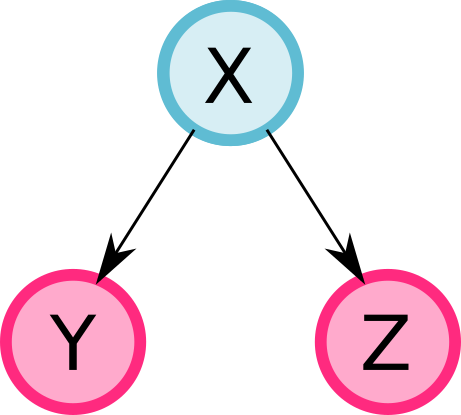
\includegraphics[scale=0.4]{Figures/ex1.png}
\end{figure}
\begin{figure}[h]
	\centering
	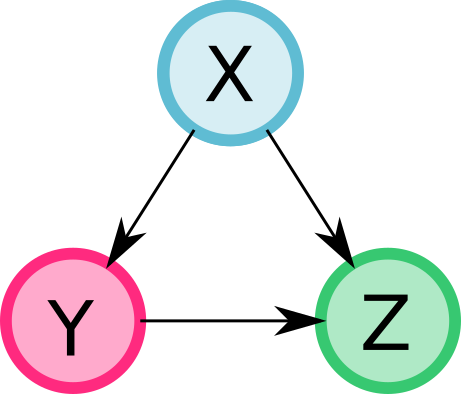
\includegraphics[scale=0.4]{Figures/ex2.png}
\end{figure}

Nullam semper quam at ante convallis posuere. Ut faucibus tellus ac massa luctus consectetur. Nulla pellentesque tortor et aliquam vehicula. Maecenas imperdiet euismod enim ut pharetra. Suspendisse pulvinar sapien vitae placerat pellentesque. Nulla facilisi. Aenean vitae nunc venenatis, vehicula neque in, congue ligula.

Pellentesque quis neque fringilla, varius ligula quis, malesuada dolor. Aenean malesuada urna porta, condimentum nisl sed, scelerisque nisi. Suspendisse ac orci quis massa porta dignissim. Morbi sollicitudin, felis eget tristique laoreet, ante lacus pretium lacus, nec ornare sem lorem a velit. Pellentesque eu erat congue, ullamcorper ante ut, tristique turpis. Nam sodales mi sed nisl tincidunt vestibulum. Interdum et malesuada fames ac ante ipsum primis in faucibus.

\begin{figure}[h]
	\centering
	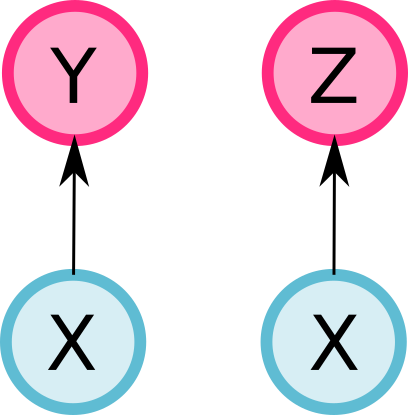
\includegraphics[scale=0.4]{Figures/ex1input.png}
\end{figure}
\begin{figure}[h]
	\centering
	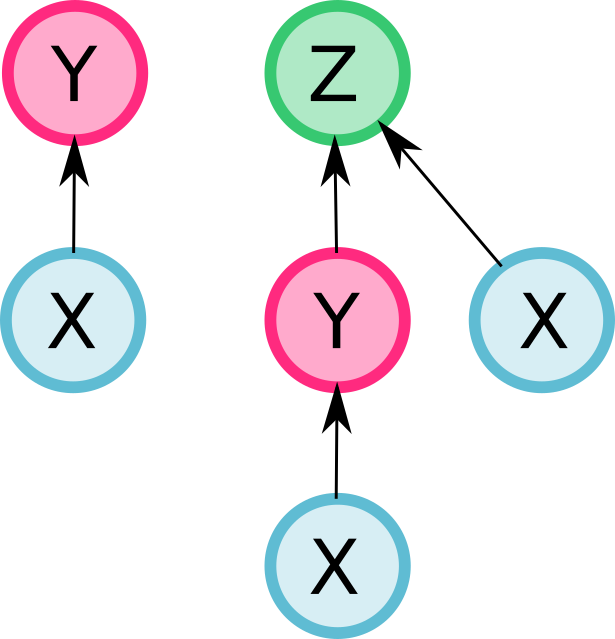
\includegraphics[scale=0.4]{Figures/ex2input.png}
\end{figure}

%------------------------------------------------

\section{\textit{Coarsest Refinement Partitioning }Algorithm}

In order to identify the correct distribution of network fibers we have to find a efficient procedure to split the network in different disjoint partitions, in which all nodes from a same partition should receive information from the same other partitions. To do that, we treat our problem as the same of find the coarsest relational refinement partitioning for the given network. In this section, we detail the optimal algorithm used to find this coarsest partitioning in a context of graph fibrations and show the relative simple implementation of this method.

\subsection{Algorithm description}

The algorithm used in this project is a slightly modified version of the algorithm presented by Paige and Tarjan \cite{Tarjan1987}, \ having a time complexity of $O(M\log N)$, being very efficient for sparse networks. This algorithm has the same runtime order than the algorithm from Cardon and Crushemore \cite{Cardon1982}, but it has a simpler implementation and smaller prefactors, exhibiting a better approach to our problem. Even though the algorithm applies for general situations, here we give the details of the algorithm to its application for a network, so we introduce the necessary definitions within this context.

A network $G$ is completely defined as $G(V, E)$ by the sets of nodes $V$ and of the connections $E$. The network has then $N = |V|$ nodes that can have connections with one another defined by the set $E$ containing $M = |E|$ ordered pair of nodes, denoting the directed connections between the network nodes. Over the network, we can define a graph partition $P$ of $V$ as a set of pairwise disjoints subsets of $V$ whose union is all $V$
\begin{equation}
	P = \cup_{i=1}^{N_P} P_i
\end{equation}
where $P_i$ are the elements of the partition $P$, in which we call it blocks. Within this context, if we consider an additional graph partition $Q$ that has the property that all the block of $Q$ is contained in a block of $P$, we say that $Q$ is a refinement partition of $P$.

Considering a block $B$ in $P$, we say that the block $B$ is stable with respect with a set $S$ if or all elements of $B$ connects an element of $S$ or none element of $B$ points to any element of $S$. By that we define that a graph partition $P$ of $V$ is stable if it is stable with respect with its own blocks. Having defined that, the graph coarsest partition problem is that of finding, for a given set of connections $E$ and initial partition $P$ over $V$, the coarsest stable refinement of $P$. 

Considering all that, for the proper identification of the fibers on the network we have to construct a stable graph partition that is equivalent to the coarsest (minimal number of blocks) refinement of the network with respect to the information flow passing through each node. For that, we need to extend the concept of stability over the partition for one that accounts for the information received by each block of the partition. Thus, in order to identify the clusters with isomorphic input-tree for all their nodes, we require that the partition should be not only stable but input-tree stable. That means that for a subset $S \subseteq$ $V$, a graph partition $P$ over the network $G(V, E)$ is input-tree stable with respect to $S$ if for all the block $B \in P$, the equality
\begin{equation}
	| E^{-1}(\{x\}) \cap S | = | E^{-1}(\{y\}) \cap S |
\end{equation}
is satisfied for all the elements $x$, $y \in B$.

This way, we can benefit from the stability properties \cite{Tarjan1987} to construct a refinement algorithm step that can obtains, through a finite number of steps, a input-tree stable partition from an initial unstable partitioning of the network. With this, given a subset $S \subseteq V$, the refinement step has the effect to refine the current partition, unstable with respect to $S$, by replacing it for a new partition now stable with $S$. For that, we define a split function \textit{I-split($S$, $P$)} that receive as input the current partition and a set $S$ and results as output a new input-tree stable partition with respect to $S$. That function benefits from two major properties of stability (and input-tree stability): the stability inheritance by refinement and by union of sets. Since this refinement inheritance, a given set $S$ can be used only once by the function \textit{I-split}, for which after all other refinement will be stable with respect to $S$. Moreover, since stability is inherited under union of sets $S$, after sets are used in \textit{I-split}, their union cannot be used for the function. With all this considered, the essence of the algorithm can be stated as

\begin{quotation}
	Find a set $S$ in which the current partition $P$ is input-tree unstable. Replace $P$ by the output of \textit{I-split($S$,$P$)}. Guarantees that the set $S$ or unions of used sets never be used again.
\end{quotation}

Since the finest partitioning possible is the one in which every node is itself a block, the refinement step can be proceeded at most $N-1$ times, guaranting that the algorithm terminates with the correct answer, since stability is inherited by the refinement process. However, to guarantees that the algorithm has a optimal runtime we have to find a efficient way to select the appropriate sets to the refinement step, without choosing repeated sets. Fortanately, this can be easily done for the construction of a input-tree stable partition.

Given a set $S$ of nodes from the network $G$ and a given input-tree unstable graph partition $Q$, the blocks $B \in Q$ that are input-tree unstable with respect to $S$ can be splitted in several blocks $B_j$ to have a stable input-tree for $S$. Then, each splitted block will have the property defined by
\begin{equation}
	B_j = \{ x \in B : | E^{-1}(\{x\}) \cap S | = j \}
\end{equation}
where the number of splitted block must be larger than one to a proper split process take place. Then, for each unstable block $B \in Q$ all the splitted block, except the largest one, can be put a queue to be used ahead in the algorithm as a refinement set. This ensures that none repeated sets or union of repeated sets can be used during the algorithm exeecution.

Having said all that, the complete algorithm to find the correct network fibers of a network $G(V, E)$ consists in initializing a graph partition $Q$ over all nodes from $V$ except the nodes that do not receive information from any other node, in which each one of these will be defined as isolated fibers already in the beginning of the algorithm. The partition $Q$ is defined as one block containing all the other nodes in the network. The algorithm maintains a queue $L$ of possible refinement sets, initially containing the single block of $Q$ and all the isolated blocks defined at the beginning. Then, we proceed as
\begin{quotation}
	Remove from $L$ its first set $S$. Replace $Q$ by the \textit{I-split($S$, $Q$)}. Whenever a block $B \in Q$ splits into two or more nonempty blocks, add all but the largest to the back of $L$.
\end{quotation}
And this process is repeated until the queue $L$ is empty. At this point, the resulted partition $Q$ represent the coarsest input-tree stable partitioning of the network $G(V, E)$, where each block represents a network fiber with all its nodes having isomorphic input-trees.

% faltou o preprocessing.

\subsection{Data preparation and algorithm implementation}

We apply the above algorithm in the genetic regulatory network of the \textit{Escherichia Coli} bacteria. We obtain the genetic E. Coli network through its transcriptional regulatory interactions data, where each gene is regulated by a transcription factor protein. Since a transcription factor production in the cell is regulated by a gene, we can define a directed connection between two genes if a gene regulates the production of a transcriptional factor, which it regulates another gene. Since a transcription factor can be either an activator(positive) or repressor(negative), or even behaves as both(dual), the links between genes can carry different types of messages. Because of that, it is important that the partitioning algorithm accounts the type of message to construct appropriate input-trees for the network fibers partition. Therefore, for a proper application of the algorithm on the \textit{Escherichia Coli} genetic network, we label each node uniquely, either as number or string names, and also each link with the type of connection between genes.

Considering this context, we explain now how the algorithm should proper be implemented to have an optimal perfomance concerning its runtime complexity. After discussing the data structures necessary to deal correctly with data, we design an algorithm recipe to show all the main steps of the process explained above. Also, anyone can acess our own personal implementation for genetic regulatory networks in the link \url{https://github.com/higorsmonteiro/fiberblocks} on github platform.

Given a directed network $G(V, E)$ to be partitioned in fibers, it is very important for the correctness of the algorithm that the nodes that do not receive any information, that is, the nodes that do not have any inward connections, be preprocessing as isolated blocks. This means that the initial graph partition $P$ is divided in two different partition $P'$ e $P''$, the first one contained all the single-node blocks containing the solitaire nodes $v$ in which $| E^{-1}(\{v\}) | = 0$, and the second one containing initialing a single block containing all the other nodes $w$ in which $| E^{-1}(\{w\}) | \geq 1$. The importance of this preprocessing is to guarantee that solitaire nodes do not be put on the same fibers during the refinement steps. Even though the blocks of $P'$ are used as refinement sets, $P'$ is not used by the algorithm. Thus, the final partition is the union of $P'$ and the result of the refinement partitioning of $P''$.

After the above preprocessing we define the data structures for the partition $Q$ for its blocks $B$. A partition is a doubly linked list of blocks, which allows that deletion of blocks be made in constante time $O(1)$ as long we have the block memory address during the procedure. A block is just a structure containing indexing data along with a doubly linked list containg all the nodes that belongs to it. Together with a queue of blocks $L$, these constructions are the main data structures necessary for an efficient implementation of the refinement partitioning algorithm. At the beginning of the algorithm, we enqueue all the blocks of $P'$ e $P''$ to $L$. Then, we start the algorithm initializing a partition $Q = P''$ and by removing the top element set $S$ of $L$, then we apply the \textit{I-split($S$, $Q$)} to identify the input-tree unstable blocks of $Q$ and split them into input-tree stable blocks with respect to  $S$. This way, all the splitted blocks are push to the end of $L$, with exception the largest resulted blocks for each splitted block. As we have mentioned, the algorithm terminates when there is no more sets in $L$. Even though this is the whole algorithm, the implementation of the \textit{I-split} function is not so straightforward, since a given block $B$ can be splitted into an arbitrary number of blocks. So, we detail the implementation of this function below.

In the algorithm recipe below, the structures $U$ and $S$ are initially empty partitions and are used to store, respectively, all the input-tree unstable blocks of $Q$ and all the splitted blocks from $U$.

\begin{algorithm}
   \caption{Input-tree split function}
    \begin{algorithmic}[1]
      \Function{\textit{I-split}}{$S, Q$}
        \State Initialize the empties partitions $U, T$
        \For{$\forall B \in Q$}
			\For{$\forall x \in B$}
            	\State Calculates $| E^{-1}(\{x\})\cap S |$
			\EndFor 
			\If {$| E^{-1}(\{x\})\cap S | \neq | E^{-1}(\{y\})\cap S |$} \Comment{$x, y \in B$}
				\State insert block $B$ in $U$.
			\EndIf       
		\EndFor
        \For{$\forall B \in U$}
			%\State defines an empty partition $Z$
			\For{$\forall x \in B$}
				\If{$\exists \ X \in T : | E^{-1}(\{x\})\cap S | = T(E)$ }
					\State insert $x$ in $X$
				\Else				
					\State create a new block $X$
					\State insert $x$ in $X$
					\State $X(E) \leftarrow | E^{-1}(\{x\})\cap S |$
					\State insert block $X$ in $T$ 
				\EndIf
			\EndFor
			\State enqueue all blocks $X \in T$ to $L$, except $Larger(T)$
        \EndFor
       \EndFunction

\end{algorithmic}
\end{algorithm}

%------------------------------------------------

\section*{Results}

Fusce in nibh augue. Cum sociis natoque penatibus et magnis dis parturient montes, nascetur ridiculus mus. In dictum accumsan sapien, ut hendrerit nisi. Phasellus ut nulla mauris. Phasellus sagittis nec odio sed posuere. Vestibulum porttitor dolor quis suscipit bibendum. Mauris risus lectus, cursus vitae hendrerit posuere, congue ac est. Suspendisse commodo eu eros non cursus. Mauris ultrices venenatis dolor, sed aliquet odio tempor pellentesque. Duis ultricies, mauris id lobortis vulputate, tellus turpis eleifend elit, in gravida leo tortor ultricies est. Maecenas vitae ipsum at dui sodales condimentum a quis dui. Nam mi sapien, lobortis ac blandit eget, dignissim quis nunc.

Donec luctus tincidunt mauris, non ultrices ligula aliquam id. Sed varius, magna a faucibus congue, arcu tellus pellentesque nisl, vel laoreet magna eros et magna. Vivamus lobortis elit eu dignissim ultrices. Fusce erat nulla, ornare at dolor quis, rhoncus venenatis velit. Donec sed elit mi. Sed semper tellus a convallis viverra. Maecenas mi lorem, placerat sit amet sem quis, adipiscing tincidunt turpis. Cras a urna et tellus dictum eleifend. Fusce dignissim lectus risus, in bibendum tortor lacinia interdum.

\begin{table}[h] % [h] forces the table to be output where it is defined in the code (it suppresses floating)
	\caption{Example table.}
	\centering
	\begin{tabular}{l l r}
		\toprule
		\multicolumn{2}{c}{Name} \\
		\cmidrule(r){1-2}
		First Name & Last Name & Grade \\
		\midrule
		John & Doe & $7.5$ \\
		Richard & Miles & $5$ \\
		\bottomrule
	\end{tabular}
\end{table}

Fusce eleifend porttitor arcu, id accumsan elit pharetra eget. Mauris luctus velit sit amet est sodales rhoncus. Donec cursus suscipit justo, sed tristique ipsum fermentum nec. Ut tortor ex, ullamcorper varius congue in, efficitur a tellus. Vivamus ut rutrum nisi. Phasellus sit amet enim efficitur, aliquam nulla id, lacinia mauris. Quisque viverra libero ac magna maximus efficitur. Interdum et malesuada fames ac ante ipsum primis in faucibus. Vestibulum mollis eros in tellus fermentum, vitae tristique justo finibus. Sed quis vehicula nibh. Etiam nulla justo, pellentesque id sapien at, semper aliquam arcu. Integer at commodo arcu. Quisque dapibus ut lacus eget vulputate.

\section{Conclusion}

Nullam semper quam at ante convallis posuere. Ut faucibus tellus ac massa luctus consectetur. Nulla pellentesque tortor et aliquam vehicula. Maecenas imperdiet euismod enim ut pharetra. Suspendisse pulvinar sapien vitae placerat pellentesque. Nulla facilisi. Aenean vitae nunc venenatis, vehicula neque in, congue ligula.


%----------------------------------------------------------------------------------------
%	BIBLIOGRAPHY
%----------------------------------------------------------------------------------------

\bibliographystyle{unsrt}

\bibliography{sample.bib}

%----------------------------------------------------------------------------------------

\end{document}
